% v13 --- Problem, Introduction, and the switched model. Owner's plan,
% 2026-09-04:
%   * the PROBLEM is bullet facts 1/2/3 answering "why must it switch", drawn
%     from docs/EECON49_[Nui](1).md section 1;
%   * the INTRODUCTION page carries Figure 1 from docs/source/figures plus the
%     m_i equation;
%   * the NEXT page carries Figure 2 plus the state vectors X_sys, x_IBR, x_SG,
%     x_GFL, x_GFM;
%   * the cover's title box takes the same colour as the top and bottom bars.
% Nothing else yet -- this is v13's whole scope.
%
% FIGURE NUMBERING follows the source paper's own, which is why Figure 1 is the
% electrical model and Figure 2 the control structure: the red dashed box inside
% Figure 1 points at "รูปที่ 2", and with this order that pointer still lands on
% the right page.
%
% COVER COLOUR. Measured from the v12 render: the frametitle bar is
% myblue!82!black = RGB(0,0,146), the footline was Berlin's own RGB(38,38,134),
% and the cover box was RGB(51,51,178) -- three different blues. All three are
% now myblue!82!black, so "same as the top and bottom bars" is true of the bars
% themselves as well, not just of the cover.
\documentclass{beamer}
\usepackage{fontspec}
\setsansfont[Path=C:/Users/User/AppData/Local/Microsoft/Windows/Fonts/,UprightFont=Helvetica.ttf,BoldFont=Helvetica-Bold.ttf,ItalicFont=Helvetica-Oblique.ttf,BoldItalicFont=Helvetica-BoldOblique.ttf]{Helvetica.ttf}
\usetheme{Berlin}
\usefonttheme[onlymath]{serif}
\usepackage{xcolor}
\usepackage{graphicx}
\usepackage{amsmath,amsfonts,amssymb}
\usepackage{bm}
\setcounter{MaxMatrixCols}{20}
\usepackage{booktabs,array,multicol}
\usepackage{tikz}
\usetikzlibrary{arrows.meta,positioning,shapes}

\definecolor{myblue}{rgb}{0.0,0.0,0.7}
\definecolor{pnavy}{HTML}{0F2A4A}
\definecolor{pblue}{HTML}{1D5288}
\definecolor{pgreen}{HTML}{1E7E34}
\definecolor{pred}{HTML}{A93226}
\definecolor{pyellow}{HTML}{B7950B}
% The one bar colour, used by the frametitle, the footline and the cover box.
\colorlet{barblue}{myblue!82!black}

\setbeamercolor{item}{fg=myblue}
\setbeamercolor{block title}{bg=barblue,fg=white}
\setbeamercolor{block body}{bg=blue!7,fg=black}
\setbeamercolor{itemize item}{fg=myblue}
\setbeamertemplate{navigation symbols}{}
\setbeamercolor{frametitle}{bg=barblue,fg=white}
\setbeamertemplate{section in toc}[sections numbered]
\setbeamertemplate{background}{}
\setbeamertemplate{headline}{}
% Numbered figures and equations, per the standing rule: every figure and every
% equation must carry a number so it can be pointed at during questions.
%
% CAPTIONS ARE CENTRED AND SAY WHAT THE FIGURE IS, nothing more (owner, 2026-09-05):
% Beamer's default caption template is a flush-left paragraph, which on a one-line
% caption reads as a stray sentence under the artwork. This template centres it and
% keeps the numbered label inline. Findings belong in the talk, not under the picture.
\setbeamertemplate{caption}[numbered]
\setbeamertemplate{caption}{\centering\insertcaptionname~\insertcaptionnumber:
  \insertcaption\par}
\setbeamerfont{caption}{size=\scriptsize}
\setbeamercolor{caption name}{fg=barblue}
% Berlin's footline draws its own two colour boxes in author/date colours. Both
% are set to barblue so the strip matches the frametitle exactly.
\setbeamercolor{author in head/foot}{bg=barblue,fg=white}
\setbeamercolor{date in head/foot}{bg=barblue,fg=white}
\setbeamertemplate{footline}{%
  \leavevmode%
  \hbox{%
  \begin{beamercolorbox}[wd=.88\paperwidth,ht=2.6ex,dp=1.1ex,leftskip=1.2em]{author in head/foot}%
    \ifodd\insertframenumber\relax
      \scriptsize An Automatic Following/Forming Framework for Inverter-Based Resources%
    \else
      \scriptsize Department of Electrical Engineering, School of Engineering, KMITL%
    \fi
  \end{beamercolorbox}%
  \begin{beamercolorbox}[wd=.12\paperwidth,ht=2.6ex,dp=1.1ex,center]{date in head/foot}%
    \scriptsize \insertframenumber/\inserttotalframenumber
  \end{beamercolorbox}}%
}

\newcommand{\pu}{\,\mathrm{p.u.}}

% The two status marks of the summary page. Drawn in tikz rather than set from a
% symbol font: fontspec loads Helvetica for text, which carries neither a tick nor a
% ballot box, and amssymb's \checkmark would arrive in a different typeface from every
% other glyph on the slide. baseline pulls the box onto the text baseline so a row of
% the table does not sit low.
\newcommand{\ckbox}{\tikz[baseline=-0.055cm]{%
  \draw[line width=0.6pt,pgreen] (0,0) rectangle (0.26,0.26);
  \draw[line width=1.0pt,pgreen] (0.055,0.145) -- (0.115,0.062) -- (0.215,0.205);}}
\newcommand{\opbox}{\tikz[baseline=-0.055cm]{%
  \draw[line width=0.6pt,black!55] (0,0) rectangle (0.26,0.26);}}

\begin{document}

% ========================= 1. COVER =====================================
% The title box is barblue, the same colour as the frametitle and footline bars.
\begin{frame}[plain]
\centering
\vspace{0.75cm}
\begin{beamercolorbox}[wd=0.86\paperwidth,sep=0.22cm,center]{frametitle}
{\Large\bfseries An Automatic Following/Forming Framework\\for Inverter-Based Resources}
\end{beamercolorbox}
\vspace{0.60cm}
{\fontsize{10.5}{13}\selectfont
Phichitchai Jueajan\quad 66010569\\
Pakkapol Phdungdan\quad 66010612\\[0.20cm]
Advisor: Dr. Tossaporn Surinkaew\\
Co-advisor: Prof. Dr. Issarachai Ngamroo\\[0.45cm]
Department of Electrical Engineering, School of Engineering\\
King Mongkut's Institute of Technology Ladkrabang (KMITL)
}
\end{frame}

% ========================= 2. TABLE OF CONTENTS ==========================
% Nothing is abbreviated here: the contents list is the first thing a reader
% looks at, and an abbreviation may only be used after it has been spelled out.
%
% THIS LIST IS THE NAMING AUTHORITY (owner, 2026-09-05): every frame title in the deck
% is its section's entry here, verbatim. It listed 9 entries while the deck had 12
% sections, so the three result/comparison/summary sections were invisible to a reader
% holding page 2. All twelve are listed now.
%
% Set at \large with a 1.30 stretch rather than \Large at 1.65: twelve rows at the old
% size ran past the footline, and a contents page that spills is worse than one a
% point smaller.
\begin{frame}{Table of Contents}
\centering
\renewcommand{\arraystretch}{1.30}
\begin{tabular}{c@{\hspace{0.35cm}}l}
\colorbox{barblue}{\makebox[0.48cm][c]{\color{white}\large 1}} & {\large Problem}\\
\colorbox{barblue}{\makebox[0.48cm][c]{\color{white}\large 2}} & {\large Introduction}\\
\colorbox{barblue}{\makebox[0.48cm][c]{\color{white}\large 3}} & {\large Converter and Machine States}\\
\colorbox{barblue}{\makebox[0.48cm][c]{\color{white}\large 4}} & {\large Switching Decision}\\
\colorbox{barblue}{\makebox[0.48cm][c]{\color{white}\large 5}} & {\large Power Flow and Time-Domain Simulation}\\
\colorbox{barblue}{\makebox[0.48cm][c]{\color{white}\large 6}} & {\large Case Study: IEEE 14-Bus System}\\
\colorbox{barblue}{\makebox[0.48cm][c]{\color{white}\large 7}} & {\large Scenario Timeline}\\
\colorbox{barblue}{\makebox[0.48cm][c]{\color{white}\large 8}} & {\large Result: The Index and the Mode}\\
\colorbox{barblue}{\makebox[0.48cm][c]{\color{white}\large 9}} & {\large Result: Voltage and Frequency}\\
\colorbox{barblue}{\makebox[0.48cm][c]{\color{white}\large 10}} & {\large Result: Active and Reactive Power}\\
\colorbox{barblue}{\makebox[0.48cm][c]{\color{white}\large 11}} & {\large Comparison: Adaptive against Fixed GFL}\\
\colorbox{barblue}{\makebox[0.48cm][c]{\color{white}\large 12}} & {\large Proof: The Switched Dynamics}\\
\colorbox{barblue}{\makebox[0.48cm][c]{\color{white}\large 13}} & {\large Summary}
\end{tabular}
\end{frame}

% ========================= 3. THE PROBLEM ================================
% Four bullet facts, from docs/EECON49_[Nui](1).md section 1 (บทนำ). The closing
% "the mode itself must be a decision" line is GONE by instruction -- fact 4 now
% carries that content as a fact rather than as a slogan, and it is a real
% citation from the paper's second paragraph (refs [2],[4],[7]): prior work fixes
% the switching condition or the control parameters in advance, so the decision
% is never made from the network's own condition.
\section{Problem}
\begin{frame}{Problem}
\vspace{0.45cm}
\large
\begin{enumerate}\setlength{\itemsep}{0.42cm}
  \item Converters are replacing synchronous machines, so \textbf{system inertia
        falls} and sensitivity to disturbances increases.
  \item \textbf{GFL} regulates power using PLL-based synchronisation, which can
        lead to oscillations or instability in a weak or low-inertia grid.
  \item \textbf{GFM} establishes its own voltage and frequency reference to support
        operation under these conditions.
  \item Existing work \textbf{fixes} the switching condition and the number of
        forming units in advance, rather than adapting them to network conditions.
\end{enumerate}
\end{frame}

% ========================= 4. INTRODUCTION ===============================
% Figure 1 is the file the owner supplied (figures/fig 1.png, copied to a
% space-free name because \includegraphics cannot take a path with a space).
% Its own red box already says "GFL/GFM mode switching strategy (Case 2)", so the
% caption does not repeat it.
%
% m_i IS BINARY, 0 = GFL and 1 = GFM, matching what Figure 2 already prints along
% its right edge. An earlier draft added a third value "out" for a converter
% taken out of service; that was wrong to put here. Out-of-service is a SEPARATE
% in-service flag in the code, written alongside the mode label rather than being
% one of its switching values (+ibr/eecon49_dual_mode_model.m:370-394), and it
% belongs with the converter-outage scenario, not on the page that introduces the
% mode command.
%
% WHAT WE DO DIFFERENTLY FROM THE SOURCE PAPER: the paper writes the right-hand
% side as one weighted sum, m*f_GFM + (1-m)*f_GFL. Our kernel never forms that
% sum -- it evaluates ONE branch and holds the other block's rows
% (dual_f:174-195). With m binary the two statements agree numerically, and the
% case form is the one that describes the code.
\section{Introduction}
\begin{frame}{Introduction}
% VERTICAL BUDGET: the figure is 3:1, so at 0.98 width it is about 3.6 cm tall,
% leaving roughly 3.9 cm for the caption, two displays and the closing line. The
% first pass at \small with default display skips overran by one line and the
% closing sentence landed under the footline. Fixed by \scriptsize plus explicit
% negative skips -- not by deleting the sentence, which carries the point.
\centering
\vspace{-0.10cm}
\begin{figure}
\centering
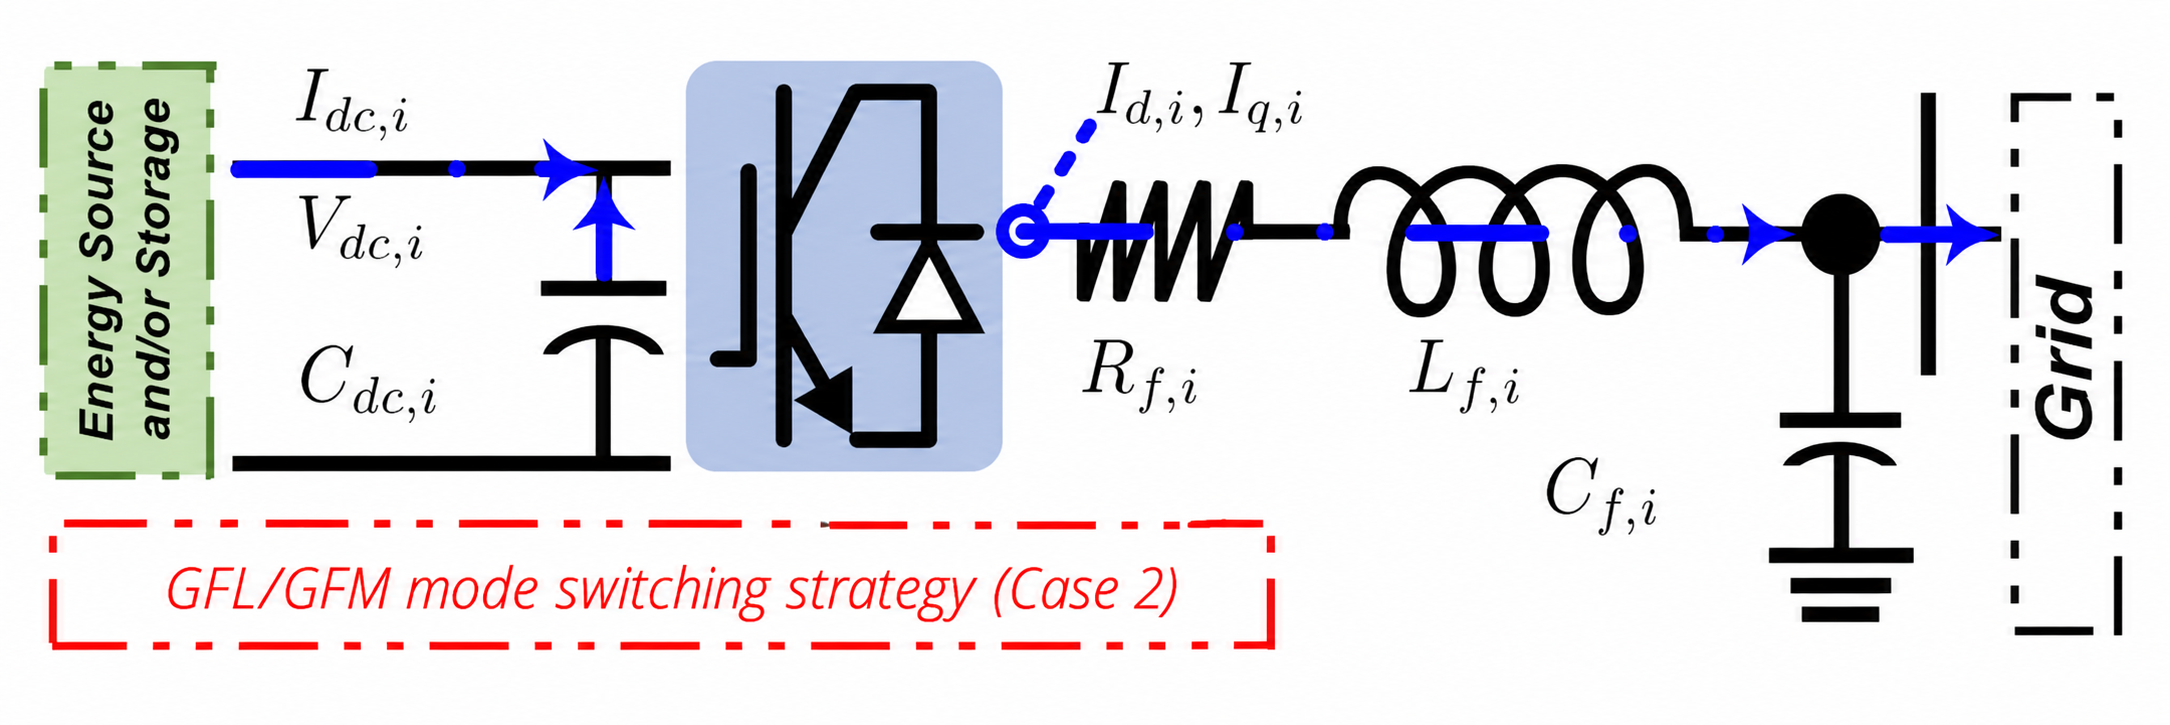
\includegraphics[width=0.98\linewidth]{figures/fig1_ibr_electrical.png}
\caption{Electrical model of one inverter-based resource (IBR).}
\label{fig:ibr}
\end{figure}

\vspace{-0.18cm}
\small
\begin{equation}
m_i(t)\in\{0,1\},\qquad 0=\text{GFL},\qquad 1=\text{GFM}
\end{equation}
\vspace{-0.30cm}
\begin{equation}
\dot{\bm x}_{IBR,i}=
\begin{cases}
\bm f_{GFL}(\bm x_{GFL},\bm y,\bm u,t), & m_i(t)=0,\\
\bm f_{GFM}(\bm x_{GFM},\bm y,\bm u,t), & m_i(t)=1.
\end{cases}
\end{equation}
\vspace{-0.14cm}

% Symbol definitions, not narration: the reader has just met x, y, u, t inside
% (2) and needs to know what each one is.
{\scriptsize
\begin{tabular}{@{}r@{\;\;}l@{\hspace{0.7cm}}r@{\;\;}l@{}}
$\bm x$ & converter and machine states &
$\bm u$ & inputs: references, loads, fault status\\
$\bm y$ & network bus voltages &
$t$ & time; events are applied at exact instants
\end{tabular}}
\end{frame}

% ================== 5. FIGURE 2 AND THE STATE VECTORS ====================
% Figure 2 is the file the owner supplied (figures/fig 2.png). It is nearly
% square (1448x1086), so it is placed BESIDE the equations rather than above
% them: at full width it left no room for the state layout.
%
% NO EQUATION NUMBERS ON THIS PAGE, by instruction. These five displays are one
% definition read top to bottom, not five results anyone will point at
% individually -- so they are align*, aligned on "=", which also buys back the
% width the number column was taking.
%
% SYMBOLS come from the models' own state names: x_SG from
% +stability/sg_composite_device.m:86, x_GFL from
% +ibr/gfl_eecon49_full_model.m:178, x_GFM from
% +ibr/gfm_eecon49_full_model.m:207.
%
% ONE HONEST NOTE ON ORDER: X_sys groups the converters first because that is the
% order asked for; the assembled vector in the code puts the SG block first. No
% index number is printed, so nothing here is falsified by that -- it is a
% reading order, not a claim about positions.
\section{Converter and Machine States}
\begin{frame}{Converter and Machine States}
\begin{columns}[c,onlytextwidth]
\column{0.50\textwidth}
\begin{figure}
\centering
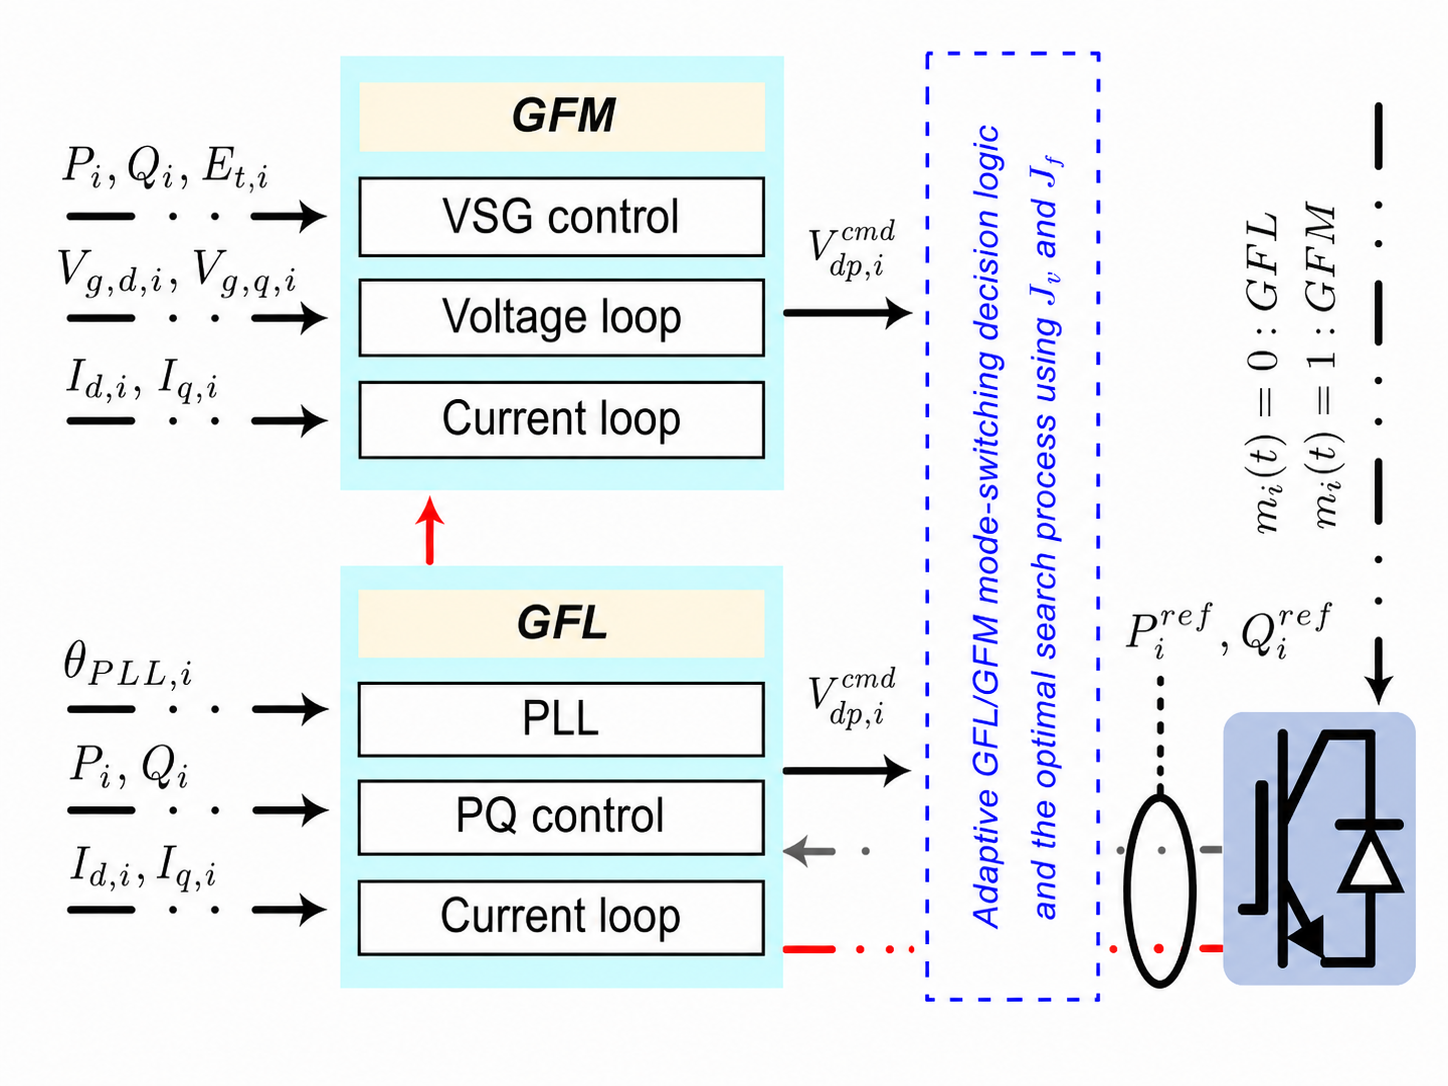
\includegraphics[width=1.00\linewidth]{figures/fig2_control_structure.png}
\caption{The two controller branches and the mode-switching decision.}
\label{fig:control}
\end{figure}
\column{0.475\textwidth}
\scriptsize
\begin{align*}
\bm X_{sys}&=\bigl[\,\bm x_{IBR,1}\;\;\cdots\;\;\bm x_{IBR,4}\;\;
  \bm x_{SG}\,\bigr]^{\!\top}\\[2pt]
\bm x_{IBR,i}&=\bigl[\,i_d,\,i_q,\,V_{dc}\;\;\bm x_{GFL}\;\;\bm x_{GFM}\;\;
  I_{dc}\,\bigr]\\[2pt]
\bm x_{SG}&=\bigl[\,\delta,\,\omega,\,e_q',\,e_d',\,e_q'',\,e_d''\,\bigr]\\[2pt]
\bm x_{GFL}&=\bigl[\,\theta_{PLL},\,\xi_{PLL},\,\xi_P,\,\xi_Q,\,\xi_{Id},\,
  \xi_{Iq}\,\bigr]\\[2pt]
\bm x_{GFM}&=\bigl[\,\theta_{VSG},\,\omega_{VSG},\,E,\,\xi_{Vd},\,\xi_{Vq},\,
  \xi_{Id},\,\xi_{Iq}\,\bigr]
\end{align*}
\vspace{-0.16cm}

{\tiny$i_d,i_q,V_{dc},I_{dc}$ are shared power-stage states integrated in both
modes. Only one of $\bm x_{GFL}$, $\bm x_{GFM}$ is integrated at a time.}
\end{columns}
\end{frame}

% ==================== 6. THE SWITCHING DECISION ==========================
% S_i built from J_V and J_f, with the 0.65 / 0.35 bands shown on an example
% trace. Requested explicitly: write the normalisation as SYMBOLS (Delta V_base,
% Delta f_base), not as the literals 0.10 and 0.50 inside the fractions, and
% state f_0 = 60 Hz.
%
% ON THE VOLTAGE REFERENCE -- one honest deviation from "V_0 = 1 pu". The code
% references each converter to ITS OWN bus's healthy power-flow magnitude
% (settings.healthy_pf_V, used at +stability/agsi_reference_terms.m:186), not to a
% flat 1 pu. That is deliberate and measured: buses 6 and 8 sit above 1 pu in the
% healthy profile, so a flat 1 pu would make J_V report standing severity while
% the system is perfectly normal. The slide therefore writes V_i^* and says in one
% line that it comes from the power flow and is close to 1 pu. Writing V_0 = 1 pu
% in the fraction would describe an index we do not run.
%
% THE TRACE IS A SCHEMATIC, and the caption says so. It is drawn to show the
% mechanism -- crossing, dwell, flip, and the deliberately asymmetric dwell times
% -- not to report a measured run. The up-dwell is drawn 10x shorter than the
% down-dwell because that is the real ratio (0.10 s against 1.00 s); labelling a
% measured-looking curve with invented numbers is the thing being avoided here.
\section{Switching Decision}
\begin{frame}{Switching Decision}
% LAYOUT, rebuilt from measurements (see the note above): equations LEFT at their
% natural amsmath spacing, schematic RIGHT scaled to its column, and the symbol
% list plus the parameter values in a FULL-WIDTH band beneath both columns.
\abovecaptionskip=1pt \belowcaptionskip=0pt
\vspace*{-0.60cm}
\begin{columns}[t,onlytextwidth]
\column{0.44\textwidth}
\vspace{0.30cm}
\scriptsize
\setlength{\jot}{0.14cm}
\begin{equation}
J_{V,i}(t)=\frac{\bigl|\,|V_i(t)|-V_i^{\star}\,\bigr|}{\Delta V_{base}}
\end{equation}
\begin{equation}
J_{f}(t)=\frac{\bigl|\,f_{coi}(t)-f_0\,\bigr|}{\Delta f_{base}}
\end{equation}
\begin{equation}
S_i(t)=\operatorname{sat}_{[0,1]}\!\bigl(w_V J_{V,i}+w_f J_f\bigr)
\end{equation}
\begin{align}
0\to1:&\quad S_i\ge\Gamma_{on}\ \text{for}\ T_{d,on}\\
1\to0:&\quad S_i\le\Gamma_{off}\ \text{for}\ T_{d,off}
\end{align}

\column{0.56\textwidth}
\begin{figure}
\centering
% xscale, not scalebox: the picture measures 197.34pt wide against this column's
% 172.08pt, so its horizontal extent has to come down -- but its LETTERING does
% not. At xscale=0.86 the box is 171.60pt wide, it keeps its full 120.24pt
% height, and every label stays at \tiny instead of 0.86 x \tiny.
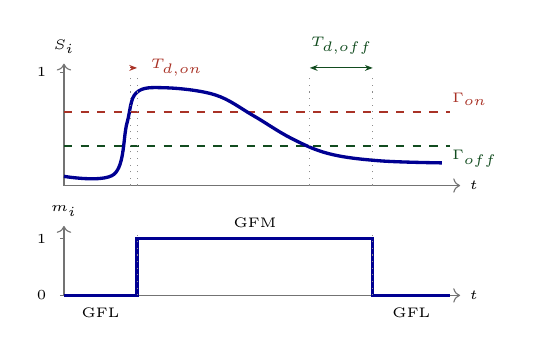
\begin{tikzpicture}[font=\tiny,xscale=0.86,yscale=0.90]
% ---- panel (a): the severity trace -------------------------------------
% Axis: 6 s -> 5.58 cm (0.93 cm/s); S in [0,1] -> 1.6 cm.
\draw[->,draw=black!55] (0,0) -- (5.85,0) node[right,font=\tiny]{$t$};
\draw[->,draw=black!55] (0,0) -- (0,1.72) node[above,font=\tiny]{$S_i$};
\draw[draw=black!55] (-0.06,1.60) -- (0,1.60) node[left,font=\tiny,xshift=-1mm]{$1$};
% the two bands
\draw[pred,dashed,thick] (0,1.04) -- (5.70,1.04)
  node[right,font=\tiny,pred,xshift=-1mm,yshift=1.6mm]{$\Gamma_{on}$};
\draw[pgreen!60!black,dashed,thick] (0,0.56) -- (5.70,0.56)
  node[right,font=\tiny,pgreen!60!black,xshift=-1mm,yshift=-1.6mm]{$\Gamma_{off}$};
% the trace
\draw[barblue,very thick] plot[smooth,tension=0.6] coordinates
  {(0,0.13) (0.74,0.16) (0.93,0.88) (1.07,1.31) (1.49,1.38) (2.23,1.28)
   (2.79,0.99) (3.35,0.67) (3.91,0.45) (4.65,0.35) (5.58,0.32)};
% crossing instants and the dwell that follows each
\draw[black!45,dotted] (0.98,0) -- (0.98,1.55);
\draw[black!45,dotted] (1.08,0) -- (1.08,1.55);
\draw[black!45,dotted] (3.63,0) -- (3.63,1.55);
\draw[black!45,dotted] (4.56,0) -- (4.56,1.55);
\draw[-{Stealth[length=1mm]},pred] (0.98,1.66) -- (1.08,1.66);
\node[font=\tiny,pred,anchor=west] at (1.14,1.66) {$T_{d,on}$};
\draw[{Stealth[length=1mm]}-{Stealth[length=1mm]},pgreen!60!black]
  (3.63,1.66) -- (4.56,1.66);
\node[font=\tiny,pgreen!60!black,anchor=south] at (4.10,1.72) {$T_{d,off}$};

% ---- panel (b): the resulting mode -------------------------------------
% Dropped to -1.55 cm: at -1.30 the "m_i" axis label of this panel landed on the
% Gamma_off rule of the panel above it.
\begin{scope}[yshift=-1.55cm]
\draw[->,draw=black!55] (0,0) -- (5.85,0) node[right,font=\tiny]{$t$};
\draw[->,draw=black!55] (0,0) -- (0,0.98) node[above,font=\tiny]{$m_i$};
\draw[draw=black!55] (-0.06,0.80) -- (0,0.80) node[left,font=\tiny,xshift=-1mm]{$1$};
\draw[draw=black!55] (-0.06,0) -- (0,0) node[left,font=\tiny,xshift=-1mm]{$0$};
\draw[barblue,very thick] (0,0) -- (1.08,0) -- (1.08,0.80) -- (4.56,0.80)
  -- (4.56,0) -- (5.70,0);
\node[font=\tiny,anchor=south] at (2.82,0.82) {GFM};
\node[font=\tiny,anchor=north] at (0.54,-0.04) {GFL};
\node[font=\tiny,anchor=north] at (5.13,-0.04) {GFL};
\draw[black!45,dotted] (1.08,0) -- (1.08,0.86);
\draw[black!45,dotted] (4.56,0) -- (4.56,0.86);
\end{scope}
\end{tikzpicture}
\caption{Mode switching on the severity index.}
\label{fig:switch}
\end{figure}
\end{columns}

% ---- the full-width band: what the symbols are, then what they are set to ----
% Both were in the left column before, at \tiny, wrapping. Here they have the
% whole 307.29pt of text width, so both are \scriptsize and neither wraps.
\vspace{0.12cm}
{\scriptsize\renewcommand{\arraystretch}{1.35}
\begin{tabular*}{\textwidth}{@{}r@{\;\,}l@{\extracolsep{\fill}}r@{\;\,}l@{}}
$J_{V,i}$ & voltage deviation of bus $i$ &
$S_i$     & severity of converter $i$, in $[0,1]$\\
$J_{f}$   & frequency deviation &
$\Gamma$  & switching threshold on $S_i$\\
$V_i^{\star}$ & bus $i$'s healthy power-flow $|V|$ &
$T_d$     & required duration beyond the threshold
\end{tabular*}}

\vspace{0.18cm}
\hrule height 0.4pt width \textwidth
\vspace{0.16cm}
{\scriptsize\renewcommand{\arraystretch}{1.35}
\begin{tabular*}{\textwidth}{@{\extracolsep{\fill}}llll@{}}
$f_0=60$~Hz & $\Delta V_{base}=0.10\pu$ & $\Delta f_{base}=0.50$~Hz &
$w_V=w_f=\tfrac12$\\
$\Gamma_{on}=0.65$ & $\Gamma_{off}=0.35$ & $T_{d,on}=0.10$~s &
$T_{d,off}=1.00$~s
\end{tabular*}}
\end{frame}

% ============ 7. POWER FLOW AND TIME-DOMAIN SIMULATION ===================
% ONE frame, two columns -- PF left, TS right.
%
% EQUATIONS VERIFIED against the code and against outside sources, 2026-09-04.
%
% PF, equations (9)-(10). What our solver actually forms is
%   mismatch_i = P_spec(i) - P_calc(i),  P_spec = P_gen - P_load
% (internal/core/pf_calculate_mismatch.m:17-21 and pf_prepare_case.m:53-54), with
%   P_calc(i) = V_i * sum_j V_j (G_ij cos d_ij + B_ij sin d_ij)
%   Q_calc(i) = V_i * sum_j V_j (G_ij sin d_ij - B_ij cos d_ij)
% (pf_calculate_power_injections.m:15-19). That is the standard convention --
% JuliaGrid's AC power-flow tutorial states net injection as production minus
% consumption, P_i = P_pi - P_di with P_pi the sum of units at the bus, and gives
% the same two Ybus sums; PowerModels states the same nodal balance in complex
% form. So the slide's rows are the code's rows with the generation term split
% into machine plus converters, which is what a converter bus needs shown.
%
% The FIRST draft of these rows was wrong in one way worth recording: it wrote
% P_j^{net} without saying what it was, which reads as "line losses" rather than
% "the Ybus injection at bus j". It is now written P_j(y) and defined.
%
% TS, equations (13)-(14). Implicit trapezoidal on the differential rows with the
% algebraic row held at the new point. Confirmed twice: our own report states
% [x_1 - x_0 - (h/2)(f_0 + f_1)]_A = 0 together with g(x_1,V_1) = 0
% (report_ieee14_switch_th_rev2.tex:1173-1179), and arXiv:2008.03883 gives the
% same discretisation as 0 = (x_t - x_{t-h}) - 0.5h(f_t + f_{t-h}) plus the
% constraint row. The one simplification: our trapezoidal row applies to the
% INTEGRATED coordinates only (the SG's E_d' is frozen), which the symbol block
% now says rather than the slide silently implying all of x.
%
% LAYOUT: equation numbers must sit beside their equation, not wrap. Both columns
% are \scriptsize with \footnotesize math bodies, and the long PF rows use short
% superscripts (G, L) instead of SG/load. Both Symbols blocks are wrapped in
% fixed-height minipages so the two blocks are the same height.
\section{Power Flow and Time-Domain Simulation}
\begin{frame}{Power Flow and Time-Domain Simulation}
\begin{columns}[t,onlytextwidth]

% ------------------------------- PF ------------------------------------
\column{0.475\textwidth}
\centering
{\small\textbf{Power-flow operating point}}
\scriptsize
% Fixed-height equation region, same value in both columns: the PF side carries
% three display rows and the TS side four, so without this the left block floats
% one row higher than the right and the two blocks do not line up.
\begin{minipage}[t][3.65cm][t]{\linewidth}
\centering
\begin{equation}
\bm 0=\bm g(\bm x,\bm y,\bm u_0,\bm m)
\end{equation}
\vspace{-0.24cm}

Power must balance at every bus $j$:
\vspace{-0.10cm}
\begin{align}
\bigl(P_j^{G}+P_j^{inj}\bigr)-P_j^{L}-P_j(\bm y)&=0\\
\bigl(Q_j^{G}+Q_j^{inj}\bigr)-Q_j^{L}-Q_j(\bm y)&=0
\end{align}
\end{minipage}
\begin{block}{Symbols}
\begin{minipage}[t][2.30cm][t]{\linewidth}
\raggedright
{\tiny
\begin{tabular}{@{}r@{\;\;}p{0.68\linewidth}@{}}
$P_j^{G},Q_j^{G}$ & machine injection at bus $j$\\
$P_j^{inj},Q_j^{inj}$ & \textbf{specified} converter injection\\
$P_j^{L},Q_j^{L}$ & load at bus $j$\\
$\bm u_0$ & fixed inputs at the operating point\\
$P_j(\bm y),Q_j(\bm y)$ & network injection with fixed $\bm Y_{bus}(\bm u_0)$\\
$|V_j|,\theta_j$ & \textbf{calculated} bus voltage
\end{tabular}}
\end{minipage}
\end{block}

% ------------------------------- TS ------------------------------------
\column{0.475\textwidth}
\centering
{\small\textbf{Time-domain response}}
\scriptsize
\begin{minipage}[t][3.65cm][t]{\linewidth}
\centering
\begin{align}
\dot{\bm x}&=\bm f\bigl(\bm x,\bm y,\bm u,\bm m,t\bigr)\\
\bm 0&=\bm g\bigl(\bm x,\bm y,\bm u,\bm m,t\bigr)
\end{align}
\vspace{-0.24cm}

One step $t_n\!\to\!t_{n+1}$ of size $h$:
\vspace{-0.10cm}
\begin{align}
\bm x_{n+1}&=\bm x_n+\tfrac{h}{2}\bigl[\bm f_n+\bm f_{n+1}\bigr]\\
\bm 0&=\bm g_{n+1}
\end{align}
\end{minipage}
\begin{block}{Symbols}
\begin{minipage}[t][2.30cm][t]{\linewidth}
\raggedright
{\tiny
\begin{tabular}{@{}r@{\;\;}p{0.68\linewidth}@{}}
$\bm x$ & converter and machine states\\
$\bm y$ & bus voltages\\
$\bm u(t)$ & references, loads and fault status\\
$\bm m(t)$ & converter modes that \textbf{change} over time\\
$h$ & step size, $t_{n+1}-t_n$\\
$\bm f_n,\bm g_n$ & (11)--(12) evaluated at\\
 & $(\bm x_n,\bm y_n,\bm u_n,\bm m_n,t_n)$\\
 & (13) applies to the integrated coordinates
\end{tabular}}
\end{minipage}
\end{block}
\end{columns}
\end{frame}

% ==================== 8. THE IEEE 14-BUS CASE ============================
% "Which bus carries the SG, which buses carry the IBRs" -- so the page is the
% supplied network drawing plus a table that answers exactly that, and nothing
% more.
%
% EVERY NUMBER ON THIS PAGE IS FROM THE CASE FILE, and the supplied drawing
% agrees with it:
%   * SG at bus 1, IBRs at buses 2/3/6/8, and the printed apparent powers
%     SG1 = 134.62 MVA, IBR = [36.31 33.02 50.86 30.64] MVA
%     (+cases/case_ieee14bus_eecon49_switch.m:6-8, and S_ibr_pu at :74).
%   * The load labels in the drawing are the IEEE-14 loads of
%     +cases/case_matpower6_case14.m:14-27. Recomputed as |S| per bus they are
%     25.14 (2), 96.10 (3), 7.77 (5), 13.48 (6), 33.85 (9), 10.71 (10),
%     3.94 (11), 6.31 (12), 14.69 (13), 15.72 (14) MVA -- the drawing's numbers
%     to the last digit. Bus 4 also carries load, 47.96 MVA, and the drawing
%     shows its arrow but prints no number; the table's total includes it.
%     259.0 MW and 73.5 MVAr over 11 buses in total.
%   * 20 branches, three of them with off-nominal taps: 4-7 (0.978), 4-9 (0.969)
%     and 5-6 (0.932) (case_matpower6_case14.m:42-44).
%
% NAMING, stated rather than smoothed over: the drawing labels the converters
% IBR_1..IBR_4 by position, our code names each one by its OWN BUS -- IBR2, IBR3,
% IBR6, IBR8 (+cases/scenario_ieee14_1sg_4ibr.m:115-118). Both appear in the
% table so a reader of the code and a reader of the slide land on the same device.
%
% BUS TYPES. In the original IEEE-14 data buses 2, 3, 6 and 8 are PV generator
% buses (case_matpower6_case14.m:15,16,19,21 type 2). This case RE-TYPES all four
% to PQ (case_ieee14bus_eecon49_switch.m:87-91, bus type 3 with the mapped P/Q),
% because a grid-following converter is a current source that does not hold its
% terminal voltage. Bus 1 is therefore the only slack bus, and its |V| setpoint is
% 1.00 pu at angle 0 (:40-41), not MATPOWER's 1.06.
\section{Case Study: IEEE 14-Bus System}
\begin{frame}{Case Study: IEEE 14-Bus System}
\vspace{-0.10cm}
\begin{columns}[c,onlytextwidth]
\column{0.575\textwidth}
\begin{figure}
\centering
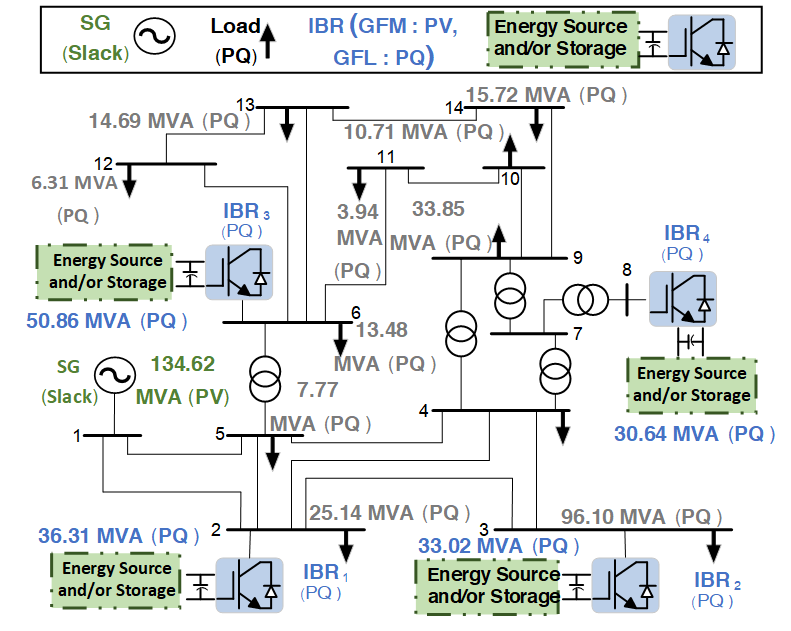
\includegraphics[width=1.00\linewidth]{figures/fig4_ieee14_network.png}
\caption{The IEEE 14-bus study network.}
\label{fig:network}
\end{figure}

\column{0.405\textwidth}
\scriptsize
\centering
\renewcommand{\arraystretch}{1.35}
\begin{tabular}{@{}llr@{}}
\toprule
Resource & Bus & MVA\\
\midrule
SG (slack) & \textbf{1} & 134.62\\
IBR$_1$ & \textbf{2} & 36.31\\
IBR$_2$ & \textbf{3} & 33.02\\
IBR$_3$ & \textbf{6} & 50.86\\
IBR$_4$ & \textbf{8} & 30.64\\
\bottomrule
\end{tabular}
\end{columns}
\end{frame}

% ==================== 9. THE SCENARIO TIMELINE ===========================
% The owner's own timeline drawing, redrawn in tikz for THIS scenario:
%   stage 1  t=0..20 s     normal operation
%   stage 2  t=20 s        SG1 (the slack machine) trips
%   stage 3  t=20 s+       a converter takes the island angle reference
%   stage 4  t=60-60.15 s  bolted fault at bus 9
%   stage 5  t=100 s       SG1 is offered back and recloses
%   stage 6  t=160 s       end of the horizon
%
% The instants are the ones the runner schedules, not illustrative numbers:
% scripts/reporting/run_ieee14_scenario_suite.m row 5 'sg_fault_cycle160' sets
% sg_trip=20, fault_on=60, fault_clear=60.15, sg_on=100 with t_end=160.
%
% STAGE 3 IS NOT A SCHEDULED EVENT, and the ring is drawn dashed to say so. The
% supervisor decides it about T_d,on = 0.10 s after the trip; which converter
% takes the reference is read out of the trajectory. Drawing it as a solid ring
% beside the four breaker events would claim the schedule chose it.
%
% Layout: two rows of three, top row left-to-right and bottom row right-to-left
% (a boustrophedon, like the owner's drawing), with the arrows following that
% order and one connector down the right edge.
\section{Scenario Timeline}
\begin{frame}{Scenario Timeline}
\centering
\vspace{0.05cm}
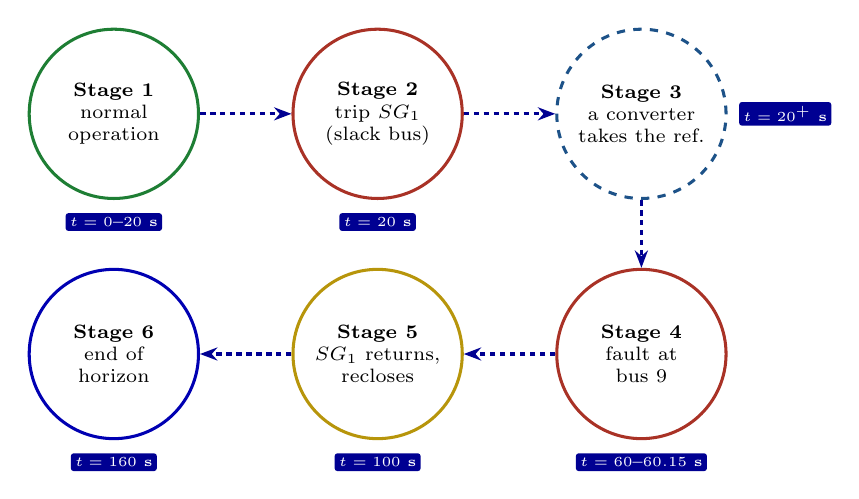
\begin{tikzpicture}[scale=1.0,every node/.style={transform shape},
  ring/.style={circle,draw,line width=1.1pt,minimum size=2.15cm,
    align=center,inner sep=1pt,font=\scriptsize},
  tstamp/.style={fill=barblue,text=white,font=\tiny\bfseries,
    inner sep=1.6pt,rounded corners=1pt},
  arr/.style={-{Stealth[length=2.2mm]},barblue,line width=1.1pt,dash pattern=on 2pt off 1.6pt}]

% ---- top row, left to right --------------------------------------------
\node[ring,draw=pgreen]              (s1) at (0.00,0)  {\textbf{Stage 1}\\normal\\operation};
\node[ring,draw=pred]                (s2) at (3.35,0)  {\textbf{Stage 2}\\trip $SG_1$\\(slack bus)};
\node[ring,draw=pblue,dashed]        (s3) at (6.70,0)  {\textbf{Stage 3}\\a converter\\takes the ref.};
% ---- bottom row, right to left -----------------------------------------
\node[ring,draw=pred]                (s4) at (6.70,-3.05) {\textbf{Stage 4}\\fault at\\bus 9};
\node[ring,draw=pyellow]             (s5) at (3.35,-3.05) {\textbf{Stage 5}\\$SG_1$ returns,\\recloses};
\node[ring,draw=myblue]              (s6) at (0.00,-3.05) {\textbf{Stage 6}\\end of\\horizon};

% ---- the instants ------------------------------------------------------
% Five stamps hang below their ring. Stage 3's sits BESIDE its ring instead: the
% top-to-bottom connector runs down that column, and a stamp below the ring cut
% it in two.
\node[tstamp,anchor=north] (t1) at ([yshift=-0.16cm]s1.south) {$t=0$--$20$ s};
\node[tstamp,anchor=north] (t2) at ([yshift=-0.16cm]s2.south) {$t=20$ s};
\node[tstamp,anchor=west]  (t3) at ([xshift=0.14cm]s3.east)   {$t=20^{+}$ s};
\node[tstamp,anchor=north] (t4) at ([yshift=-0.16cm]s4.south) {$t=60$--$60.15$ s};
\node[tstamp,anchor=north] (t5) at ([yshift=-0.16cm]s5.south) {$t=100$ s};
\node[tstamp,anchor=north] (t6) at ([yshift=-0.16cm]s6.south) {$t=160$ s};

% ---- the order ---------------------------------------------------------
\draw[arr] (s1) -- (s2);
\draw[arr] (s2) -- (s3);
\draw[arr] (s3) -- (s4);
\draw[arr] (s4) -- (s5);
\draw[arr] (s5) -- (s6);
\end{tikzpicture}
\end{frame}

% ==================== 10. THE MEASURED RESULT ============================
% The switching index and the mode it produced, both measured on the 160 s arm of
% page 9, on ONE slide. The two figures are generated on equal 4.20 x 1.38 in
% canvases at 10 pt and included at 0.86 of the text width, so the lettering
% arrives at about 9 pt -- the deck's own body size -- and both fit above the
% footline with their captions.
%
% BOTH FIGURES COME FROM ONE RUN, the cache
% output/diagnostics/ieee14_scenario_suite/sg_fault_cycle160.mat, written by
% scripts/reporting/run_ieee14_scenario_suite.m row 5 and drawn by
% scripts/reporting/generate_ieee14_agsi_mode_3d.m. That generator is a pure cache
% reader: nothing here is simulated, smoothed, decimated or re-solved at figure
% time.
%
% THE NUMBERS THE RUN REPORTED, so a caption cannot drift from them:
%   horizon 160.000000 of 160.000000 s, converged, 2288 accepted samples,
%   80 rejected steps, reclose SUCCESS at 102.3627 s, terminal f_COI 59.999958 Hz,
%   2 grid-forming intervals, 0 mode samples masked, S within [0, 1].
%
% WHAT THE TWO SAY TOGETHER: IBR_1 crosses Gamma_on just after the machine leaves
% at 20 s and holds the reference until the reclose; IBR_3 is promoted only for
% the fault window at 60 s. Both return to grid-following, which is the hand-back
% claim measured rather than asserted.
\section{Result: The Index and the Mode}
\begin{frame}{Result: The Index and the Mode}
\centering
\vspace{-0.38cm}
\begin{figure}
\centering
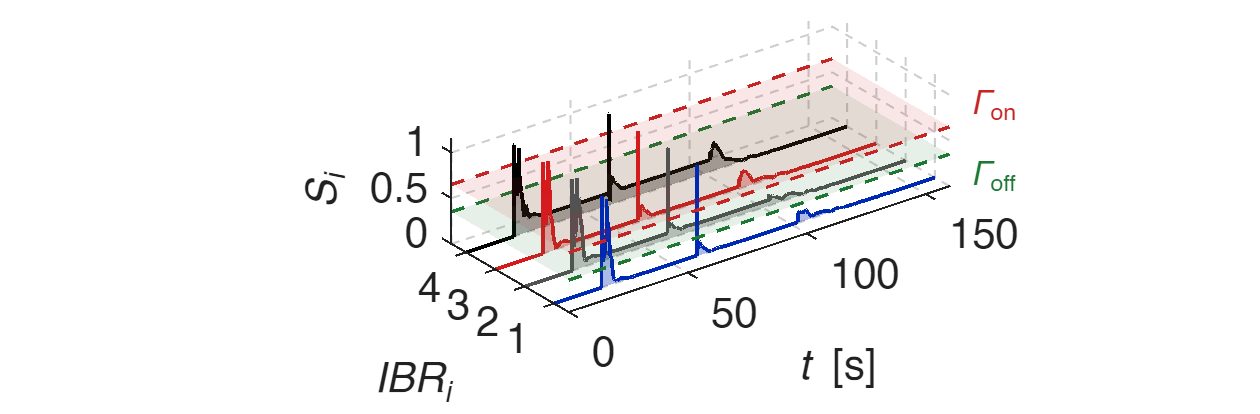
\includegraphics[width=0.86\linewidth]{figures/ieee14_scenario_suite/sg_fault_cycle160_agsi3d.png}
\caption{Switching index $S_i$ per converter.}
\label{fig:agsi}
\end{figure}

\vspace{-0.38cm}
\begin{figure}
\centering
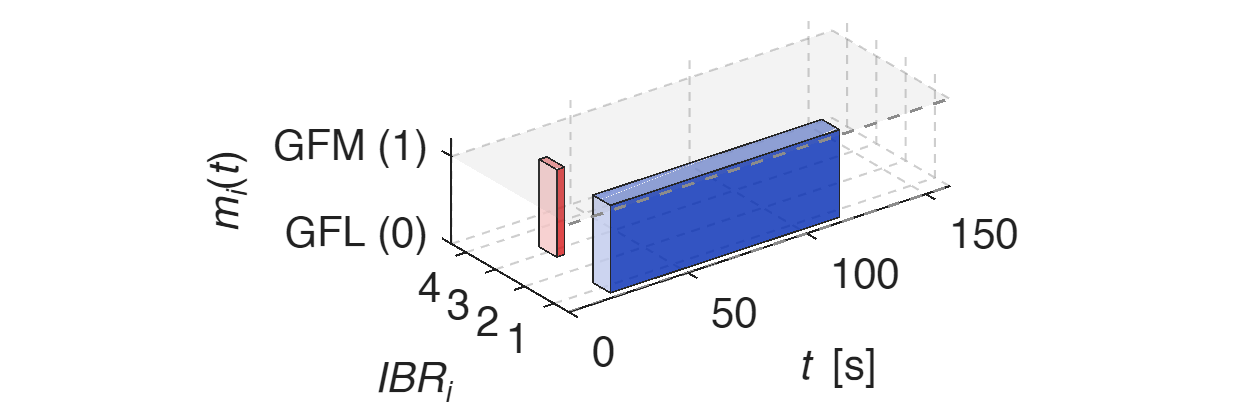
\includegraphics[width=0.86\linewidth]{figures/ieee14_scenario_suite/sg_fault_cycle160_mode3d.png}
\caption{The resulting mode $m_i(t)$ per converter.}
\label{fig:mode}
\end{figure}
\end{frame}

% ==================== 11. VOLTAGE AND FREQUENCY ==========================
% The same 160 s arm, seen in the two physical quantities: bus voltage magnitude at
% each converter and each converter's OWN frequency, each under its own "GFM Mode
% Active" strip so a feature in a trace can be attributed to a mode change without
% turning back to page 10.
%
% ONE FIGURE, generated at 4.65 x 2.90 in and included at 1:1, so the 10 pt
% lettering arrives at 10 pt -- the deck's own body size.
%
% SOURCE: the same cache as page 10,
% output/diagnostics/ieee14_scenario_suite/sg_fault_cycle160.mat, drawn by
% scripts/reporting/generate_ieee14_vf_mode_page.m.
%
% PANEL (b) IS THE CONVERTERS' OWN FREQUENCY, not the centre-of-inertia frequency.
% The run publishes device_frequency_Hz only for the machine and for a converter
% while it is grid-forming; the grid-following stretches are recovered from the
% converter's own phase-locked loop by re-evaluating the RUN'S stored device output
% map on the RUN'S stored state. Three gates hold before anything is drawn:
% reproduction of every published sample to 0.000e+00 Hz, no in-service sample left
% without a frequency, and one convention across both halves (residual 2.1e-14 Hz).
%
% NO J = 1 RULES ON EITHER PANEL and NO VERTICAL EVENT RULES, at the owner's
% instruction (2026-09-04): the dashed band edges and the dotted/dash-dot event
% rules are off the sheet. What each panel keeps is the reference its traces deviate
% FROM -- the healthy |V| per bus on (a), the nominal f_0 on (b). The two
% normalization bases are still re-derived from the plotted signals and checked
% against the run's published J_V and J_f (both residuals 0.000e+00) before the page
% draws, so it remains verified against an index it no longer shows. Every scheduled
% instant is listed in provenance_vf_mode.txt.
%
% THE NUMBERS THIS PAGE RESTS ON: |V| within [0.258, 1.864] pu over the run and
% [0.551, 1.138] pu outside the 150 ms fault window -- which is why the window is
% set on the operating band and the 1.86 pu peak is annotated at the frame instead
% of setting the axis. Converter frequency within [58.94, 60.68] Hz. 2 grid-forming
% intervals: IBR_1 from 20.00 s to 116.24 s, IBR_3 from 22.09 s to 25.30 s.
\section{Result: Voltage and Frequency}
\begin{frame}{Result: Voltage and Frequency}
\centering
\vspace{-0.24cm}
\begin{figure}
\centering
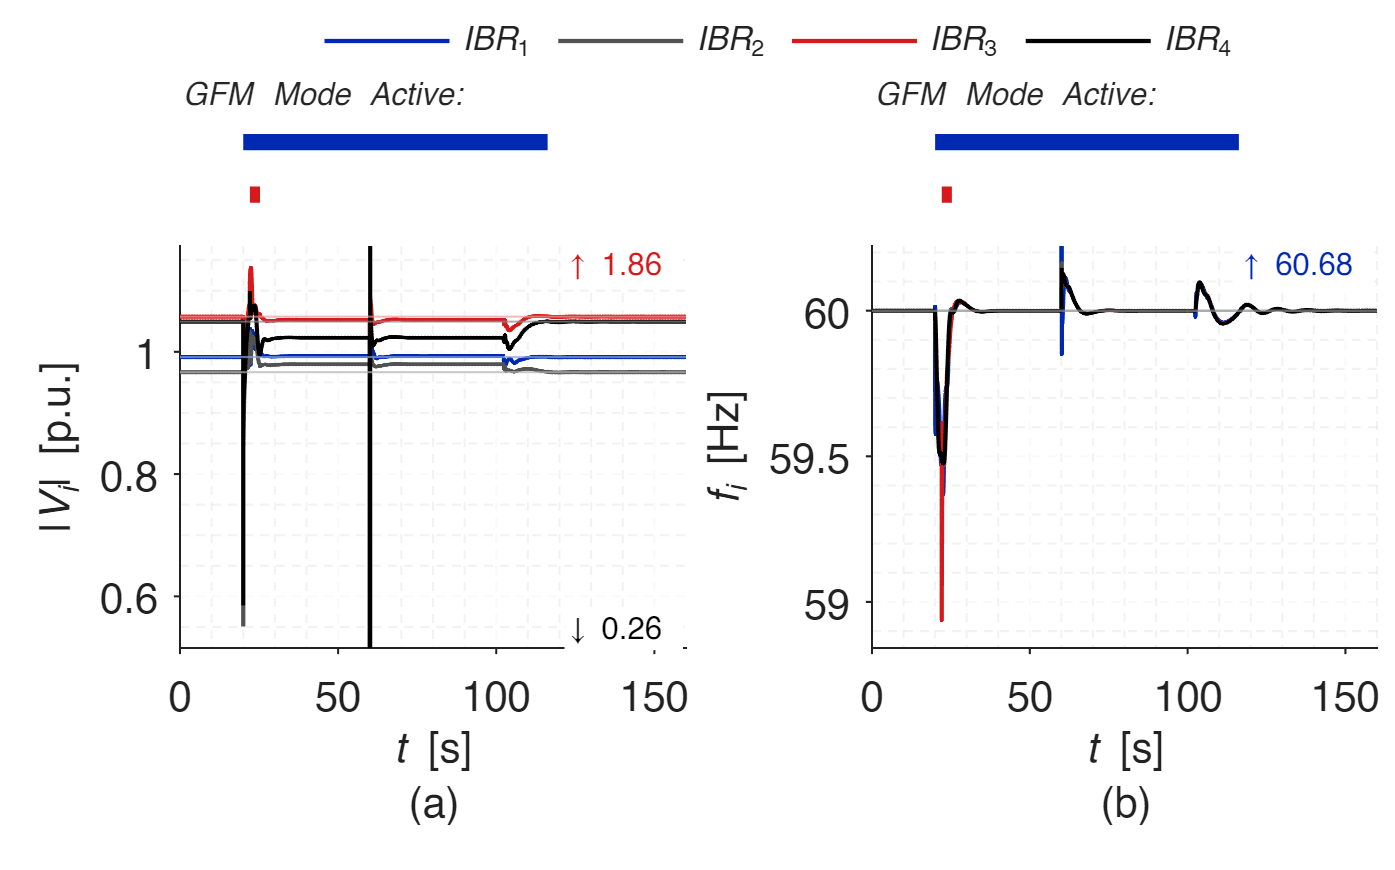
\includegraphics[width=0.95\linewidth]{figures/ieee14_scenario_suite/sg_fault_cycle160_vf.png}
\caption{(a) $|V_i|$ at each converter bus and (b) each converter's own
frequency $f_i$.}
\label{fig:vf}
\end{figure}
\end{frame}

% ==================== 12. ACTIVE AND REACTIVE POWER ======================
% The same 160 s arm again, in the two quantities the converters actually dispatch,
% laid out EXACTLY as page 11: two panels side by side, each under its own "GFM Mode
% Active" strip, so a step in a power trace can be attributed to a mode change on the
% spot. The owner asked for this page "the same as the V/f graph" (2026-09-05), so the
% canvas, the geometry, the palette, the strip, the tag placement below the x label
% and the absence of vertical event rules are all its sibling's.
%
% ONE FIGURE, generated at 4.65 x 2.90 in -- the V/f page's canvas exactly -- and
% included at 1:1, so the 10 pt lettering arrives at 10 pt and the two pages occupy
% the same rectangle.
%
% SOURCE: the same cache as pages 10 and 11,
% output/diagnostics/ieee14_scenario_suite/sg_fault_cycle160.mat, drawn by
% scripts/reporting/generate_ieee14_pq_mode_page.m. Pure cache reader: nothing is
% simulated, re-solved, smoothed, decimated or padded at figure time.
%
% NEITHER PANEL IS MASKED FOR SERVICE. The mode strip is masked -- a converter out of
% service has no mode -- but P and Q are not: a departed converter injects no current,
% so its zero is a MEASURED injection and hiding it would hide the outage. On this arm
% no converter left service, so the count of masked samples is 0.
%
% THE NUMBERS THIS PAGE RESTS ON: P within [0.041, 2.173] pu over the run but
% [0.167, 0.951] pu outside the 150 ms fault window -- the 2.17 pu peak is the
% right-limit burst of the atomic fault-clear transaction, which is why the window is
% set on the operating band and that peak is annotated at the frame instead of setting
% the axis. Q within [-0.427, 0.894] pu. 8 scheduled instants recorded, none drawn.
\section{Result: Active and Reactive Power}
\begin{frame}{Result: Active and Reactive Power}
\centering
\vspace{-0.24cm}
\begin{figure}
\centering
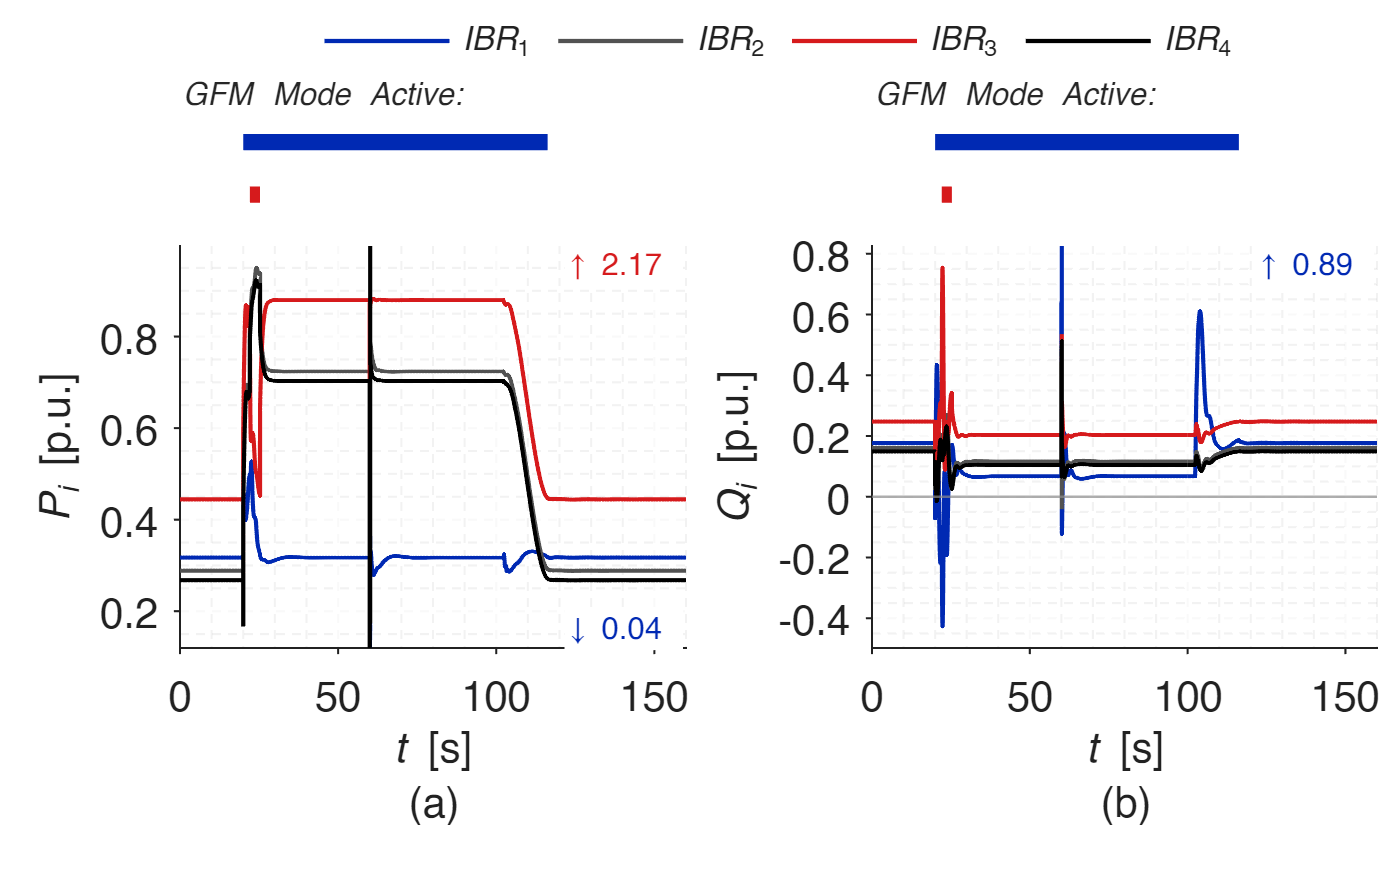
\includegraphics[width=0.95\linewidth]{figures/ieee14_scenario_suite/sg_fault_cycle160_pq_mode.png}
\caption{(a) $P_i$ and (b) $Q_i$ at each converter.}
\label{fig:pq}
\end{figure}
\end{frame}

% ==================== 13-14. THE COMPARISON, AT BUS 9 ====================
% The claim the whole deck exists to support, on TWO slides: the delivered adaptive
% GFL/GFM policy against the same case with every converter locked grid-following, at
% bus 9 -- the fault bus, which carries load but NO device, so it reports what the
% island DELIVERS to a load bus rather than what any one controller commands. One
% schedule on both arms: sg_trip 20, fault 60/60.15, sg_on 100, out to 160 s.
%
% This is the report's 2x2 bus-9 comparison figure
% (scripts/reporting/generate_bus9_adaptive_vs_fixed_160s.m) SPLIT INTO TWO PAGES of
% two panels each and restyled to match pages 11-12, at the owner's instruction
% (2026-09-05). Drawn by scripts/reporting/generate_ieee14_compare_bus9_pages.m, which
% enforces every input gate of that figure unchanged -- both classifications, both arms
% converged to 160 s, one shared event schedule, the device-to-bus mapping, one fault
% impedance, no load step, and the t=0 bus-9 identity gate (P=0.295000, Q=0.166000,
% |V|=1.021934 pu from the case load table and the PF solution) on BOTH arms.
%
% THE GREY ARM IS ASSUMED_DIAGNOSTIC, not a result: it runs with the opt-in
% allow_no_vf_island suspension and the angle_gauge_bus=1 slack pin, with a diagnostic
% PLL pair (0.20, 220). It may support a COMPARATIVE statement and never a readiness
% claim; the production noVoltageFormingSource refusal is untouched.
%
% NO MODE STRIP on these two pages, unlike 11 and 12: the strip's lanes are
% per-converter in the IBR palette, whose first hue IS this page's blue -- and here
% blue means a POLICY, not IBR_1. Each arm keeps its own accepted-sample grid (2288
% adaptive against 8007 fixed); nothing is resampled onto the other's.
%
% THE FREQUENCY PANEL IS THE FREQUENCY AT BUS 9 ITSELF, not any device's: bus 9 carries
% load but no device, so none is published for it and it is DERIVED from that bus's own
% voltage angle, f_9 = f0 + (1/2pi) d(theta_9)/dt, as the secant slope of the unwrapped
% angle across each accepted step. Both arms are derived the same way from their own
% solutions, which is what makes the panel a comparison. Four gates hold before it
% draws: the frame (before the first event both arms are synchronous, so theta_9 must be
% stationary -- measured |d theta_9| = 0 exactly, f_9 = 60.000000000 Hz), the wrap (the
% angle is unwrapped first; the fixed arm has 4318 raw wrap-sized jumps), the event jump
% (an event publishes a left and a right sample at one instant, dt = 0, and those pairs
% are dropped rather than divided by), and RESOLUTION -- a secant can only express
% |f - f0| <= 1/(2 dt), so a step whose |d theta| reaches pi/2 is not drawn. The grey
% trace is therefore BROKEN, not absent: 4488 of the fixed arm's 8006 steps are drawn
% and 3514 (70.3 s of 160) are not, because its 20 ms output grid does not resolve how
% fast that fleet moves the bus angle. The adaptive arm's own grid resolves all 2279.
%
% THE NUMBERS THESE PAGES REST ON, over the island operating band (20 <= t < 100 s
% minus the 200 ms fault window):
%   adaptive  P 0.093..0.326   Q 0.052..0.184   |V| 0.574..1.075 pu
%   fixed     P 0.000..0.563   Q 0.000..0.317   |V| 0.007..1.411 pu
% The fixed arm's |V| swings across a 1.40 pu band at a load bus; the adaptive arm holds
% 0.50 pu. On the frequency panel, over its own window (determined, off event): adaptive
% 59.27..63.62 Hz, fixed 47.53..72.50 Hz.
\section{Comparison: Adaptive against Fixed GFL}
\begin{frame}{Comparison: Adaptive against Fixed GFL}
\centering
\vspace{-0.10cm}
\begin{figure}
\centering
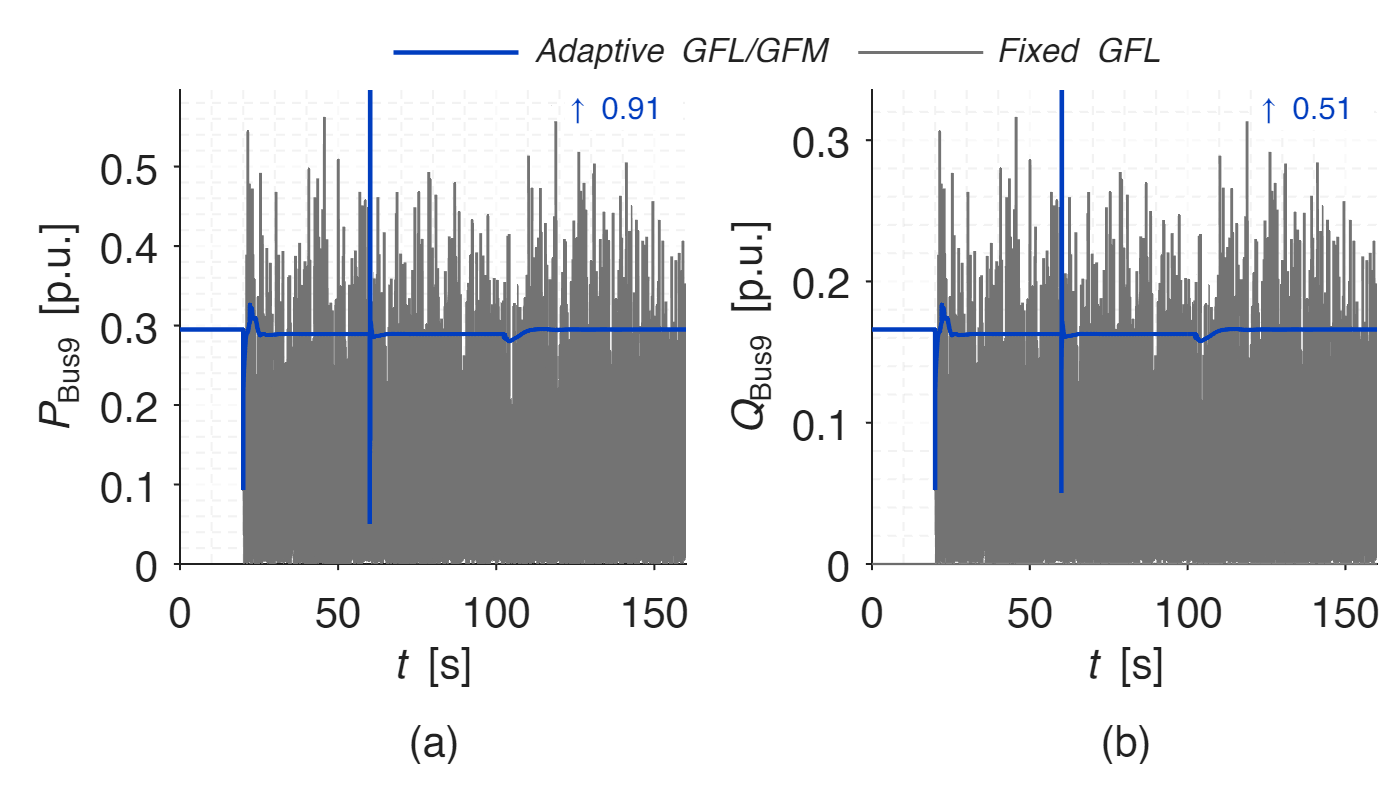
\includegraphics[width=0.95\linewidth]{figures/ieee14_scenario_suite/sg_fault_cycle160_cmp_pq.png}
\caption{(a) $P_{\mathrm{Bus9}}$ and (b) $Q_{\mathrm{Bus9}}$: adaptive (blue)
against fixed GFL (grey).}
\label{fig:cmp-pq}
\end{figure}
\end{frame}

\begin{frame}{Comparison: Adaptive against Fixed GFL}
\centering
\vspace{-0.10cm}
\begin{figure}
\centering
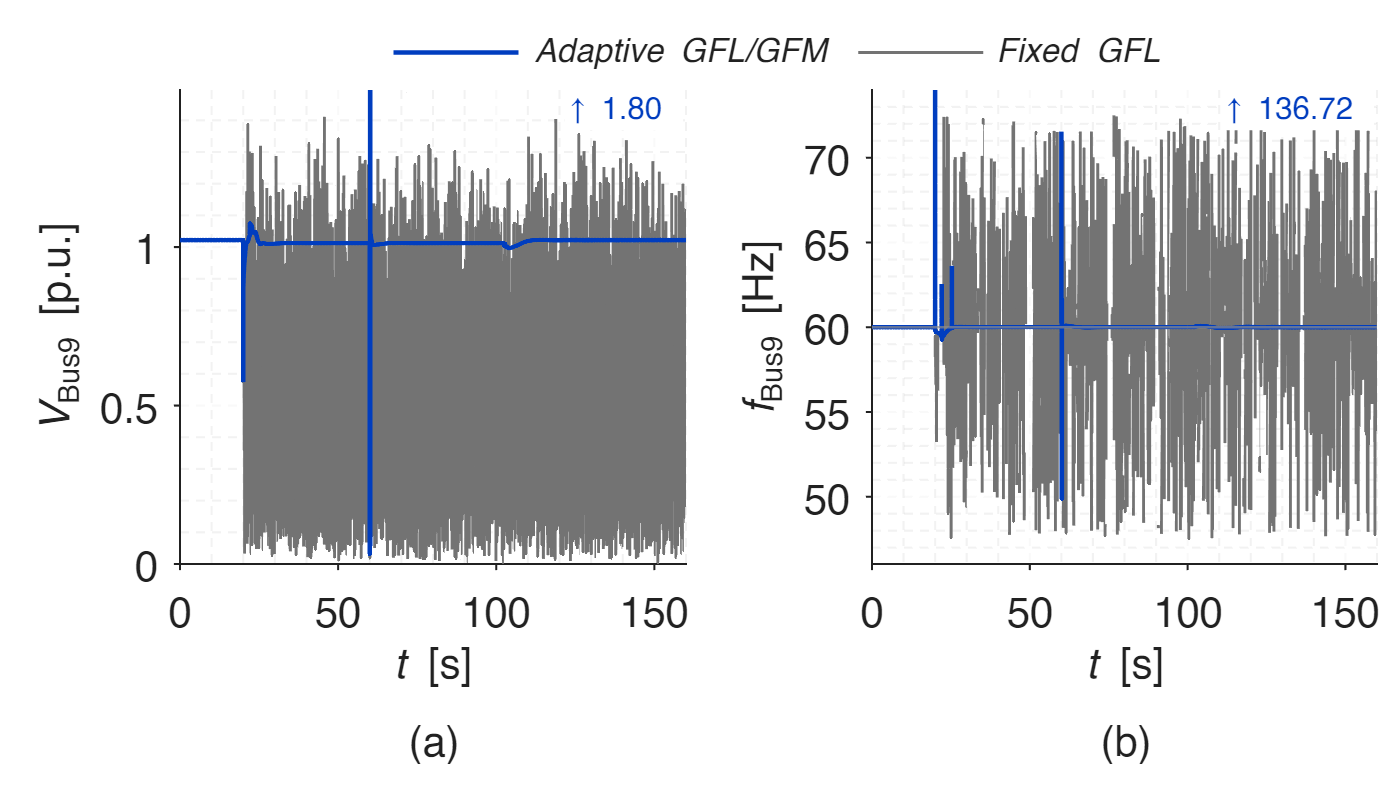
\includegraphics[width=0.95\linewidth]{figures/ieee14_scenario_suite/sg_fault_cycle160_cmp_vf.png}
\caption{(a) $V_{\mathrm{Bus9}}$ and (b) $f_{\mathrm{Bus9}}$: adaptive (blue)
against fixed GFL (grey).}
\label{fig:cmp-vf}
\end{figure}
\end{frame}

% ============ 15. PROOF: THE STACKED SWITCHED DYNAMICS ===================
% Owner, 2026-09-05, correcting the first attempt: the equation to PROVE is the
% stacked heterogeneous right-hand side -- (47) of the report --
%
%   xdot = f(x,V) = [ f_SG(x_SG,V) ; f_IBR1(x_IBR1,V;m1) ; ... ],
%       m_i in {GFL, GFM, tripped}
%
% because that is the equation in which the mode label appears, and therefore the
% equation that describes the switching event. The transfer maps are its
% corollary, not its subject.
%
% WHAT (47) ACTUALLY CLAIMS -- two things about the MODEL, not about storage:
%   (a) the composite field is the DIRECT SUM of per-device fields, each reading
%       the composite state only through its own block;
%   (b) each block reads the network only through its OWN terminal voltage.
% Both are checkable, and both were checked on the assembled system before this
% page was written (tmp/mt/probe_eq47.m; 5 devices, 74 stored states, 28
% algebraic rows, profile eecon49_figure4):
%   * df/dx by CENTRAL differences: 1192 on-block entries up to 1.005e4, and all
%     4284 OFF-block entries exactly 0, zero nonzeros. Central differences make
%     that a hard zero -- f(x+he)-f(x-he) is identically zero for a coordinate the
%     block does not read -- not a rounding artefact.
%   * df_k/dV_j over every device and every bus: own-bus sensitivity 18.4 (SG) to
%     235.2 (IBR6); every foreign-bus sensitivity exactly 0 across 5 devices and
%     13 foreign buses, zero nonzeros.
%   * flipping ONE converter's label GFL->GFM moves that converter's own rows by
%     34.4 to 177.2 and every other device's rows by exactly 0. So m_i is a
%     per-device label -- hypothesis (H3) -- and that is what makes a mode switch
%     a local event rather than a global one.
%
% THE PROOF IS ALGEBRAIC AND NEEDS NO SMOOTHNESS for part (i). With
% sum_k S_k' S_k = I one has x = sum_k S_k' x_k; differentiate, substitute the
% local law, left-multiply by S_j and use S_j S_k' = delta_jk I. That isolates
% block j as phi_j alone, which IS (47). Part (ii), the block-diagonal Jacobian,
% DOES need differentiability of each phi_k and holds pointwise only -- the
% current limiter is not differentiable on |i| = Imax -- so the slide says "where
% each phi_k is differentiable" and never claims C^1.
%
% WHY THIS ANSWERS "HOW DO WE SOLVE AN ABRUPTLY CHANGING STATE EQUATION".
% Because m_k enters only its own block and is constant between events, the
% abrupt change is confined to one block and to the instants themselves: on each
% open interval (47) is an ordinary field integrated on the active set A(m), and
% at the instant the state is re-assigned rather than integrated. Active-set
% counts measured on this very composite: 45 of 74 with four GFL converters, 49
% of 74 with four GFM, the SG contributing 5 of its 6 because E_d' is frozen at
% the singular limit.
%
% ON THE CONVERSE, left to the report: it proves the converse (block-diagonal
% Jacobian implies the local law) and exhibits f_coi as the quantity in this same
% system that WOULD break (H2) if it entered a vector field -- it enters only the
% severity index, i.e. the switching layer. The slide says only that the
% hypotheses have content.
%
% LAYOUT, priced before assembly (tmp/mt/probe_e47rows.tex): intro+(17) 49.56pt,
% hypotheses as a 2x2 grid 21.12pt (a description list was 67.73pt), the two
% displays full width 48.36pt, the proof paragraph 39.67pt, the verification
% table 41.80pt, the closing paragraph 26.82pt. Sum 227.33pt against 221.30pt of
% text height, closed by the negative leads between bands. The first attempt put
% the proof in a 0.485 column, where both displays wrapped and the column alone
% cost 142.11pt.
\section{Proof: The Switched Dynamics}
\begin{frame}{Proof: The Switched Dynamics}
% Part 1: the fixed state space and the two mode laws. u collects exogenous
% inputs, including reference and fault-status components.
%
% This frame was split out of a single over-full page (see the note above): it now
% carries the embedding alone, which is 173.60pt of the 221.30pt available, so the
% displays can keep their ordinary skips instead of the 4pt squeeze the overflow
% had forced.
\small
\setlength{\abovedisplayskip}{7pt}
\setlength{\belowdisplayskip}{7pt}
\setlength{\abovedisplayshortskip}{5pt}
\setlength{\belowdisplayshortskip}{5pt}
\vspace*{0.10cm}
{\color{barblue}\textbf{1. The same 17 states in both modes}}\par
\vspace{0.10cm}
\begin{equation}\label{eq:fixed-state-blocks}
\bm x_{IBR}=\begin{bmatrix}
\bm x_p\\ \bm x_{GFL}\\ \bm x_{GFM}
\end{bmatrix}
\quad
\begin{array}{l}
4\text{ physical states: }i_d,i_q,V_{dc},I_{dc}\\
6\text{ GFL states: PLL, PQ and current control}\\
7\text{ GFM states: VSG, voltage and current control}
\end{array}
\end{equation}
\vspace{0.10cm}
\begin{equation}\label{eq:embedded-mode-law}
\begin{aligned}
&\text{GFL }(m=0)\\[-2pt]
&\dot{\bm x}_{IBR}=\begin{bmatrix}
\bm f_p^{(0)}(\bm x,\bm y,\bm u,t)\\
\bm f_{GFL}^{c}(\bm x,\bm y,\bm u,t)\\
\bm0_7
\end{bmatrix}
\end{aligned}
\qquad
\begin{aligned}
&\text{GFM }(m=1)\\[-2pt]
&\dot{\bm x}_{IBR}=\begin{bmatrix}
\bm f_p^{(1)}(\bm x,\bm y,\bm u,t)\\
\bm0_6\\
\bm f_{GFM}^{c}(\bm x,\bm y,\bm u,t)
\end{bmatrix}
\end{aligned}
\end{equation}
\vspace{0.06cm}
{\scriptsize $\bm f_p$: physical equations. $\bm f^c$: controller equations.
$\bm0_6,\bm0_7$: inactive controller states stay constant --- they are held, not
solved, and are \emph{re-initialised} rather than continued when the mode next
becomes active.}
\end{frame}

% ---- Part 2 of the proof: the instant itself -----------------------------
% Split from the page above so neither is crowded. This frame carries the
% re-initialisation map and the one worked seed that realises it: 149.95pt of the
% 221.30pt available.
\begin{frame}{Proof: The Switched Dynamics}
\small
\setlength{\abovedisplayskip}{7pt}
\setlength{\belowdisplayskip}{7pt}
\setlength{\abovedisplayshortskip}{5pt}
\setlength{\belowdisplayshortskip}{5pt}
\vspace*{0.10cm}
{\color{barblue}\textbf{2. At $t_s$: initial states for the new mode}}\par
\vspace{0.26cm}
\textbf{The state is re-assigned, not integrated}
\begin{equation}\label{eq:hybrid-initial-condition}
\bm x^+=R(\bm x^-,\bm y^-,\bm u^-,\bm u^+),
\quad \bm g(\bm x^+,\bm y^+,\bm u^+,\bm m^+,t_s)=\bm0 .
\end{equation}
{\scriptsize $R$ sets the initial states for the chosen mode.
$-$: just before $t_s$. $+$: just after $t_s$.}

\vspace{0.34cm}
\textbf{GFL to GFM: initialize the voltage-loop state}

\vspace{0.06cm}
{\scriptsize At unchanged $V$, choose $\theta^+=\arg V$ and $E^+=|V|$.
Then $E^+-v_d^+=0$.}
\begin{equation}\label{eq:pi-initial-condition}
\xi_{Vd}^+=\frac{i_d^+}{k_{iV}}
\quad\Longrightarrow\quad
i_{d,ref}^{raw,+}=k_{pV}(0)+k_{iV}\xi_{Vd}^+=i_d^+ ,\quad k_{iV}\ne0 .
\end{equation}
\vspace{0.04cm}
{\scriptsize Likewise $\xi_{Vq}^+=i_q^+/k_{iV}$. These are matches of the
\emph{raw} reference, before current limiting.}
\end{frame}

\begin{frame}{Proof: The Switched Dynamics}
% Part 2: coordinate-invariant current matching and right-hand DAE solution.
% A bounded post-switch vector field establishes right continuity of x at x+.
% Together with the matching map this establishes physical-port continuity,
% not continuity of every controller coordinate or post-switch stability.
\small
\setlength{\abovedisplayskip}{4pt}
\setlength{\belowdisplayskip}{4pt}
\setlength{\abovedisplayshortskip}{3pt}
\setlength{\belowdisplayshortskip}{3pt}
\vspace*{-0.05cm}
{\color{barblue}\textbf{3. Continuity and the post-switch transient}}\par
{\scriptsize GFL/GFM switching with unchanged network and a locally regular DAE.
On one current base, $i_{dq}=i_d+j i_q$ and $i_s=i_{dq}e^{j\theta}$.
$\theta$ is the PLL or VSG angle.}

\vspace{0.12cm}
\textbf{The angle changes, but the physical current stays the same}
\begin{equation}\label{eq:state-matching}
i_{dq}^{+}=i_{dq}^{-}e^{j(\theta^--\theta^+)},
\qquad V_{dc}^{+}=V_{dc}^{-},\quad I_{dc}^{+}=I_{dc}^{-}.
\end{equation}
\begin{equation}\label{eq:current-matching-proof}
i_s^+=i_{dq}^+e^{j\theta^+}
=\bigl(i_{dq}^-e^{j(\theta^--\theta^+)}\bigr)e^{j\theta^+}
=i_s^- .
\end{equation}

\vspace{0.12cm}
\textbf{After $t_s$: integrate the equations of the new mode}
\begin{equation}\label{eq:post-switch-solution}
\bm x(t_s+h)=\bm x^+
+\int_{t_s}^{t_s+h}\bm f_{m^+}(\bm x(\tau),\bm y(\tau),\bm u(\tau),\tau)\,d\tau .
\end{equation}
{\scriptsize $\bm f_{m^+}$ is the new mode's state derivative.
If its magnitude stays below $B$ for the applied $\bm u(\tau)$, then}
\begin{equation}\label{eq:continuity-bound}
\|\bm x(t_s+h)-\bm x^+\|
\le Bh\xrightarrow[h\to0^+]{}0 .
\end{equation}
\begin{beamercolorbox}[wd=\textwidth,sep=0.12cm]{block body}
{\small The current is continuous, while its slope may change.\\
A transient can follow. Continuity alone does not prove stability.}
\end{beamercolorbox}
\end{frame}

% ==================== 17. SUMMARY =======================================
% The closing page the owner asked for (2026-09-05): ONE table of what was built,
% ticked where it is done and left as an EMPTY BOX where it is not, plus what the
% model buys over a fixed policy.
%
% THE TICKS ARE NOT A JUDGEMENT, they are a read of what this deck showed:
%   PF -> DAE -> SSSA -> TS on one convention   pages 5-6
%   the 17-state dual-mode converter             pages 3-4
%   the severity index and the supervisor        pages 4, 10
%   the authenticated candidate table            page 4
%   the measured 160 s full cycle                pages 9-14
%   the fixed-GFL comparison                     pages 13-14
% Every ticked row is a thing this deck put a figure or an equation behind. Nothing is
% ticked on the strength of intent.
%
% THE EMPTY BOXES are the owner's four named next items -- control gates, nonlinear
% analysis, and the rest -- drawn as open squares so the page can be ticked by hand in
% the room. They are stated as WORK, not as claims:
%   * control gates: the reclose synchronism gate exists (dV, df, dtheta) and is what
%     admits the machine back; what is NOT built is a gate on the MODE change itself --
%     the supervisor commits on the severity index plus the authenticated table, with
%     no admissibility certificate on the arriving state. AGSI-2026-08-14-01 (OPEN) is
%     exactly this: a controlled replay at one augment shows the incumbent's arriving
%     state can sit outside the basin the linear screen implied.
%   * nonlinear analysis: the candidate table is authenticated by a SMALL-SIGNAL screen
%     and then confirmed by one nonlinear run per commit. What is not built is a
%     nonlinear certificate -- a region of attraction, or a Lyapunov argument -- so the
%     screen's set and the nonlinear truth can differ, and did: the all-four-forming
%     set passes the linear screen and stops at t=25.485 s in simulation.
%   * scale: candidate enumeration is 2^n - 1 over n converters; 15 sets at n=4 is
%     exhaustive, a larger fleet is not.
%   * EMT / unbalance / grid code: this is a balanced three-phase RMS-phasor model, so
%     no grid-code compliance is claimed and none can be until protection, fault-ride-
%     through and device ratings are modelled.
%
% Kept to two columns and one closing line so it reads in one look: an 11-row table
% down the page overflowed the frame by 219 pt, and shrinking the type to fit would
% have put the closing page below the body size every other slide uses.
% LAYOUT NOTES, because this page was rebuilt three times:
%   * Every text cell is RAGGED RIGHT. Justified type in a 5 cm column opens rivers of
%     white space between words -- that is what made the first two attempts look
%     untidy, not the content.
%   * Each "Done" row is ONE claim on one or two lines; each "Next" row is a bold title
%     with a grey gloss under it. That gives the two columns similar mass, so neither
%     ends in a block of empty page.
%   * The closing statement sits in a tinted full-width box rather than as loose text,
%     so it reads as the conclusion and cannot be mistaken for a ninth table row.
%   * SIZE IS SET BY THE FRAME, not by taste: at \footnotesize the two columns plus the
%     box ran 57 pt past the footline. The tables are \scriptsize and each gloss is
%     \tiny, which is what makes the whole page fit above the bar with the closing box
%     intact -- dropping the box would have been the wrong economy.
\section{Summary}
\begin{frame}{Summary}
\vspace{0.10cm}
{\footnotesize
\begin{columns}[t,onlytextwidth]
\column{0.495\textwidth}
{\color{barblue}\textbf{Completed work}}\\[0.04cm]
{\color{barblue}\rule{\linewidth}{0.6pt}}\\[0.10cm]
\begin{tabular}{@{}c@{\hspace{0.18cm}}>{\raggedright\arraybackslash}p{0.845\linewidth}@{}}
\ckbox & Power flow and time-domain simulation\\[0.26cm]
\ckbox & GFL/GFM converter model\\[0.26cm]
\ckbox & Continuous current and DC states during mode transfer\\[0.26cm]
\ckbox & Switching based on voltage and frequency deviations\\[0.26cm]
\ckbox & Selection of grid-forming converters\\[0.26cm]
\ckbox & Comparison with fixed GFL control\\
\end{tabular}

\column{0.475\textwidth}
{\color{barblue}\textbf{Future work}}\\[0.04cm]
{\color{barblue}\rule{\linewidth}{0.6pt}}\\[0.10cm]
\begin{tabular}{@{}c@{\hspace{0.18cm}}>{\raggedright\arraybackslash}p{0.835\linewidth}@{}}
\opbox & Stability conditions for mode switching\\[0.38cm]
\opbox & Nonlinear stability analysis\\[0.38cm]
\opbox & Systems with more converters\\[0.38cm]
\opbox & EMT simulation, unbalanced operation and protection\\
\end{tabular}
\end{columns}}

\vspace{0.28cm}
\begin{beamercolorbox}[wd=\textwidth,sep=0.16cm]{block body}
{\scriptsize
The model combines GFL power regulation and GFM voltage and frequency support
in one converter. Automatic mode selection allows the converter to respond
to changing grid conditions.\par}
\end{beamercolorbox}
\end{frame}

\end{document}
